%===============================================================================
% LaTeX sjabloon voor de bachelorproef toegepaste informatica aan HOGENT
% Meer info op https://github.com/HoGentTIN/latex-hogent-report
%===============================================================================

\documentclass[dutch,dit,thesis]{hogentreport}

% - If necessary, replace the option `dit`' with your own department!
%   Valid entries are dbo, dbt, dgz, dit, dlo, dog, dsa, soa
% - If you write your thesis in English (remark: only possible after getting
%   explicit approval!), remove the option "dutch," or replace with "english".

%% Pictures to include in the text can be put in the graphics/ folder
\graphicspath{{../graphics/}}

%% For source code highlighting, requires pygments to be installed
%% Compile with the -shell-escape flag!
%% \usepackage[chapter]{minted}
%% If you compile with the make_thesis.{bat,sh} script, use the following
%% import instead:
\usepackage[section,outputdir=../output]{minted}
\usemintedstyle{solarized-light}

\usepackage{listings}
\usepackage{color}

\definecolor{dkgreen}{rgb}{0,0.6,0}
\definecolor{gray}{rgb}{0.5,0.5,0.5}
\definecolor{mauve}{rgb}{0.58,0,0.82}

\lstset{frame=tb,
  language=Java,
  aboveskip=3mm,
  belowskip=3mm,
  showstringspaces=false,
  columns=flexible,
  basicstyle={\small\ttfamily},
  numbers=none,
  numberstyle=\tiny\color{gray},
  keywordstyle=\color{blue},
  commentstyle=\color{dkgreen},
  stringstyle=\color{mauve},
  breaklines=true,
  breakatwhitespace=true,
  tabsize=3
}

% Formatting for minted environments.
\setminted{%
    autogobble,
    frame=lines,
    breaklines,
    linenos,
    tabsize=4
}

%% Ensure the list of listings is in the table of contents
\renewcommand\listoflistingscaption{%
    \IfLanguageName{dutch}{Lijst van codefragmenten}{List of listings}
}
\renewcommand\listingscaption{%
    \IfLanguageName{dutch}{Codefragment}{Listing}
}
\renewcommand*\listoflistings{%
    \cleardoublepage\phantomsection\addcontentsline{toc}{chapter}{\listoflistingscaption}%
    \listof{listing}{\listoflistingscaption}%
}

% Other packages not already included can be imported here

%%---------- Document metadata -------------------------------------------------
\author{Silas De Vuyst}
\supervisor{Dhr. T. Desmedt}
\cosupervisor{Dhr. S. Willems}
\title[]%
    {De efficiëntie van gamification bij het aanleren van COBOL aan junior developers.}
\academicyear{\advance\year by -1 \the\year--\advance\year by 1 \the\year}
\examperiod{1}
\degreesought{\IfLanguageName{dutch}{Professionele bachelor in de toegepaste informatica}{Bachelor of applied computer science}}
\partialthesis{false} %% To display 'in partial fulfilment'
%\institution{Internshipcompany BVBA.}

%% Add global exceptions to the hyphenation here
\hyphenation{back-slash back-end front-end main-frame Java-Script Type-Script
    gami-fi-ca-tion gami-fied WORK-ING-STORAGE PRO-CE-DURE-DI-VI-SION
    Octa-ly-sis sand-box}

%% The bibliography (style and settings are  found in hogentthesis.cls)
\addbibresource{bachproef.bib}            %% Bibliography file
\addbibresource{../voorstel/voorstel.bib} %% Bibliography research proposal
\defbibheading{bibempty}{}

%% Prevent empty pages for right-handed chapter starts in twoside mode
\renewcommand{\cleardoublepage}{\clearpage}

\renewcommand{\arraystretch}{1.2}

%% Content starts here.
\begin{document}

%---------- Front matter -------------------------------------------------------

\frontmatter

\hypersetup{pageanchor=false} %% Disable page numbering references
%% Render a Dutch outer title page if the main language is English
\IfLanguageName{english}{%
    %% If necessary, information can be changed here
    \degreesought{Professionele Bachelor toegepaste informatica}%
    \begin{otherlanguage}{dutch}%
       \maketitle%
    \end{otherlanguage}%
}{}

%% Generates title page content
\maketitle
\hypersetup{pageanchor=true}

%%=============================================================================
%% Voorwoord
%%=============================================================================

\chapter*{\IfLanguageName{dutch}{Woord vooraf}{Preface}}%
\label{ch:voorwoord}

Tijdens mijn opleiding Toegepaste Informatica aan HOGENT koos ik bewust voor de keuzerichting Mainframe. Daar leerde ik COBOL via uitgebreide handleidingen en klassieke colleges, terwijl ik moderne talen in de jaren ervoor net via interactieve sandboxes en gamified leerpaden had aangeleerd. Dat contrast intrigeerde me, en het werd nog scherper toen ik hoorde dat 250 miljard regels COBOL nog steeds de wereldeconomie aansturen terwijl de generatie die ze onderhoudt met pensioen gaat. Mijn eigen leerproces gaf me een goed beeld van welke COBOL-bouwstenen voor een beginner het lastigst zijn, en die ervaring werd het vertrekpunt van deze bachelorproef.

Tot slot wil ik enkele mensen bedanken. In de eerste plaats mijn co-promotor, dhr.\ S.\ Willems, wiens grondige feedback en scherpe kritische vragen op elke iteratie van dit werk de kwaliteit ervan een aanzienlijke duw in de rug hebben gegeven. Zijn blik vanuit het werkveld hielp telkens opnieuw om vage formuleringen aan te scherpen, redeneringen te onderbouwen en de scope realistisch te houden. Zonder die voortdurende kritische lezing zou deze bachelorproef niet zijn wat hij vandaag is. Daarnaast wil ik ook de docenten en medestudenten van de Mainframe-keuzerichting bedanken, die mijn COBOL-fundament hebben gelegd waarop dit werk verder bouwt. En mijn familie en vrienden, die het hele traject mee uitzaten en op de juiste momenten zorgden voor de nodige afleiding.

\bigskip
\noindent
Veel leesplezier.

\bigskip
\noindent
Silas De Vuyst \\
Gent, mei 2026

%%=============================================================================
%% Samenvatting
%%=============================================================================

%%---------- Nederlandse samenvatting -----------------------------------------
%
% Deze blok wordt enkel ingevoegd wanneer het document in het Engels wordt
% gecompileerd. Wie de bachelorproef in het Nederlands schrijft, kan dit
% negeren. De inhoud verschijnt dan niet in het document.

\IfLanguageName{english}{%
\selectlanguage{dutch}
\chapter*{Samenvatting}
\lipsum[1-4]
\selectlanguage{english}
}{}

%%---------- Samenvatting -----------------------------------------------------
% De samenvatting in de hoofdtaal van het document

\chapter*{\IfLanguageName{dutch}{Samenvatting}{Abstract}}

Wereldwijd draaien banken, overheden en zorginstellingen op honderden miljarden regels COBOL-code. Tegelijk gaan ervaren COBOL-specialisten met pensioen, terwijl er weinig nieuw talent bijkomt. Dit fenomeen wordt de \textit{silver tsunami} genoemd. Junior developers groeien op met moderne talen zoals Python en met interactieve sandboxes. Voor hen voelt COBOL dubbel vreemd. De syntax is strikt en verbose, en het bestaande leermateriaal is vooral statisch, met PDF-handleidingen en theoretische tutorials. Deze bachelorproef gaat na of \textit{gamification}, het inzetten van game-elementen in een niet-spelcontext, die instapdrempel kan verlagen.

De centrale onderzoeksvraag luidt: \textit{\enquote{Hoe effectief is gamification bij het aanleren van COBOL aan junior developers die gewend zijn aan moderne talen zoals Python?}} Vijf deelvragen behandelen de verschillen tussen COBOL en Python, de leerbarrières voor junioren, de relevante gamification-elementen, het ontwerp van een gamified leeromgeving en de verhouding tot traditionele methoden zoals een papieren cursus.

Het onderzoek verloopt in vier fasen. De eerste fase is een literatuurstudie over de mainframe-context, de verschillen tussen COBOL en Python en de gamification-frameworks PBL, MDA en Octalysis. In de tweede fase wordt een Proof-of-Concept (PoC) gebouwd, \textit{Learn COBOL}. Dat is een interactieve webapplicatie die COBOL probeert aan te leren aan junior developers door gebruik te maken van de geïdentificeerde gamification-elementen in de literatuurstudie. In de derde fase wordt de PoC geëvalueerd in twee delen. Het eerste deel is een vergelijkende literatuurevaluatie, waarin elke ontwerpkeuze wordt afgezet tegen empirisch onderzoek over gamification, programmeeronderwijs en didactiek. Het tweede deel is een uitgewerkt maar niet uitgevoerd pilotontwerp, waarin twee groepen deelnemers elk één dag COBOL leren (sectie~\ref{sec:evaluatie-pilotstudie}), de ene groep via de PoC en de andere groep via traditionele methoden. De vierde fase formuleert de conclusie en de aanbevelingen.

De literatuurevaluatie toont dat de ontwerpkeuzes aansluiten bij wat in de geraadpleegde bronnen staat. De meta-analyse van \textcite{Zhan2022} rapporteert voor gamification in programmeeronderwijs medium-tot-grote effectgroottes (\(SMD \approx 0{,}77\) op motivatie en \(\approx 0{,}75\) op academische prestaties). Omdat de PoC meerdere van die kerncomponenten implementeert (punten, badges, levels, directe feedback en sociale vergelijking), is het aannemelijk dat een pilot effecten in dezelfde grootteorde kan tonen. Dit blijft een verwachting, want er zijn geen metingen op deelnemers uitgevoerd. De PBL-triade wordt verspreid toegepast, in lijn met de waarschuwing van \textcite{KevinWerbach2020} dat leaderboards niet voor iedereen even motiverend werken. In het Octalysis-model van \textcite{Chou2015} domineren de \textit{White Hat}-drijfveren (CD1 tot CD3), die op langetermijnbetrokkenheid mikken. De \textit{Black Hat}-elementen (CD6 tot CD8) worden bewust spaarzaam ingezet.

De toegevoegde waarde voor het werkveld is viervoudig. Er is een theoretisch kader dat gamification (PBL, MDA en Octalysis) koppelt aan mainframe-onderwijs. Er is een functionele Proof-of-Concept op moderne webtechnologie (React, TypeScript, Supabase en Monaco). Er is een uitgevoerde literatuurevaluatie die per ontwerpkeuze onderbouwt waarom het ontwerp aannemelijk is. Tot slot is er een uitgewerkt pilotontwerp dat als blauwdruk voor empirische validatie kan dienen. De belangrijkste beperkingen worden in de bachelorproef expliciet benoemd. Een literatuurevaluatie stelt geen empirische geldigheid voor de PoC zelf vast. De meta-analyses gaan vooral over moderne talen en niet over COBOL. De voornaamste aanbeveling is de uitvoering van het pilotontwerp uit sectie~\ref{sec:evaluatie-pilotstudie}.


%---------- Inhoud, lijst figuren, ... -----------------------------------------

\tableofcontents

% In a list of figures, the complete caption will be included. To prevent this,
% ALWAYS add a short description in the caption!
%
%  \caption[short description]{elaborate description}
%
% If you do, only the short description will be used in the list of figures

\listoffigures

% If you included tables and/or source code listings, uncomment the appropriate
% lines.
\listoftables

\listoflistings

%%=============================================================================
%% Lijst van afkortingen
%%=============================================================================

\chapter*{\IfLanguageName{dutch}{Lijst van afkortingen}{List of abbreviations}}%
\label{ch:afkortingen}
\addcontentsline{toc}{chapter}{\IfLanguageName{dutch}{Lijst van afkortingen}{List of abbreviations}}

\begin{description}[leftmargin=3.5cm,labelwidth=3cm,style=nextline,font=\bfseries]
    \item[BMC]      BMC Software, leverancier van mainframe-managementsoftware en bron van het jaarlijkse \textit{Mainframe Survey} rapport.
    \item[CD]       Core Drive, één van de acht psychologische motivatoren binnen het Octalysis-framework van \textcite{Chou2015}.
    \item[CICS]     Customer Information Control System, IBM-transactieserver voor mainframe-applicaties.
    \item[COBOL]    Common Business Oriented Language, procedurele programmeertaal, oorspronkelijk uit 1960, nog steeds dominant op mainframes.
    \item[CRUD]     Create, Read, Update, Delete, standaardoperaties op een datastore.
    \item[DB2]      Database 2, relationele database van IBM, courant gekoppeld aan COBOL-applicaties op z/OS.
    \item[DV]       Deelvraag, in dit document genummerd DV1 t.e.m.\ DV5 (zie sectie~\ref{sec:onderzoeksvraag}).
    \item[ECB]      European Central Bank.
    \item[IBM]      International Business Machines, historische ontwikkelaar van het mainframe-platform en van \textit{Enterprise COBOL for z/OS}.
    \item[IDE]      Integrated Development Environment.
    \item[ING]      ING Group, internationale bank-/verzekeringsgroep, voorbeeld van een grote COBOL-gebruiker.
    \item[JCL]      Job Control Language, scriptingtaal voor het inplannen van batchjobs op IBM-mainframes.
    \item[MDA]      Mechanics, Dynamics, Aesthetics, formeel framework voor game-design van \textcite{Hunicke2004}.
    \item[OOP]      Object-Oriented Programming, object-georiënteerd programmeren.
    \item[PBL]      Points, Badges, Leaderboards, de meest bekende componenten van gamification \autocite{KevinWerbach2020}.
    \item[PDF]      Portable Document Format, in dit document ook de gebruikte vormgeving van de traditionele leerconditie (``PDF-pack'').
    \item[PIC]      \texttt{PICTURE}-clausule in COBOL, definieert opslagformaat en datatype van een variabele.
    \item[PoC]      Proof of Concept, tastbaar prototype dat de haalbaarheid van een idee demonstreert.
    \item[RAS]      Reliability, Availability, Serviceability, kernkwaliteitsattributen van mainframe-platformen \autocite{Ebbers2011}.
    \item[RLS]      Row-Level Security, rij-gebaseerde toegangscontrole, hier op niveau van Supabase/PostgreSQL.
    \item[RPG]      Report Program Generator, andere legacy-taal van IBM, vooral op AS/400 en IBM~i.
    \item[SMD]      Standardised Mean Difference, gestandaardiseerd gemiddeld verschil, een effectgroottemaat in meta-analyses.
    \item[SUS]      System Usability Scale, tien-item Likert-vragenlijst voor de bruikbaarheid van een systeem (vermeld als aanbeveling voor empirische opvolging).
    \item[TI]       Toegepaste Informatica, opleiding aan HOGENT waaruit deze bachelorproef voortkomt.
    \item[UI]       User Interface, gebruikersinterface.
    \item[z/OS]     IBM-besturingssysteem voor de mainframe-familie System z.
\end{description}


%---------- Kern ---------------------------------------------------------------

\mainmatter{}

% De eerste hoofdstukken van een bachelorproef zijn meestal een inleiding op
% het onderwerp, literatuurstudie en verantwoording methodologie.
% Aarzel niet om een meer beschrijvende titel aan deze hoofdstukken te geven of
% om bijvoorbeeld de inleiding en/of stand van zaken over meerdere hoofdstukken
% te verspreiden!

\input{inleiding}
\input{standvanzaken}
\input{methodologie}

% Voeg hier je eigen hoofdstukken toe die de ``corpus'' van je bachelorproef
% vormen. De structuur en titels hangen af van je eigen onderzoek. Je kan bv.
% elke fase in je onderzoek in een apart hoofdstuk bespreken.

%%=============================================================================
%% Proof Of Concept
%%=============================================================================


% ==============================================POC============================================== %
\chapter{\IfLanguageName{dutch}{Proof of Concept}{Proof of Concept}}%
\label{ch:poc}

Dit hoofdstuk beschrijft de concrete uitwerking van de Proof of Concept (PoC): een webapplicatie genaamd \textit{Learn COBOL} die COBOL-concepten aanreikt via een gamified leerpad, gekoppeld aan de Python-achtergrond van de doelgroep.
De PoC is het tastbare artefact uit fase~2 van de methodologie (zie hoofdstuk~\ref{ch:methodologie}) en dient als basis voor de gebruikersevaluatie (interviews, observaties).

\section{Doel en afbakening}

\subsection{Functionele doelstelling}
De applicatie moet junior developers op een gestructureerde manier laten kennismaken met typische COBOL-bouwstenen die in de literatuurstudie als drempelvormend naar voren kwamen: divisions, \texttt{PIC}-clausules, datahiërarchie, conditionele logica, iteraties, paragrafen en een eerste contactpunt met foutafhandeling rond bestanden (\texttt{FILE STATUS}).
In plaats van een volledige compileromgeving wordt bewust gekozen voor \textbf{heuristische validatie}: de gebruiker krijgt per level een checklist van doelen; voldoet de ingediende code aan die patronen, dan wordt het level als geslaagd beschouwd.

\subsection{Niet-doelen van de PoC}
Om de scope beheersbaar te houden voor het onderzoek, behoren tot de bewuste \textit{niet-doelen}:
\begin{itemize}
    \item \textbf{Geen uitvoering van COBOL op een mainframe of in een echte runtime:} er wordt geen batchjob of transactieserver gevoed.
    \item \textbf{Geen volledige taaldekking:} slechts zeven thematische levels; edge cases en dialectverschillen worden niet afgedekt.
    \item \textbf{Geen formele correctheidsbewijs:} regex-gebaseerde checks kunnen zowel false positives als false negatives vertonen; de nadruk ligt op didactiek en motivatie, niet op certificerende nauwkeurigheid.
\end{itemize}

\section{Technische architectuur en technologiekeuzes}

\subsection{Client: React, TypeScript en Vite}
De front-end is gebouwd met \textbf{React~18} en \textbf{TypeScript}, gebundeld met \textbf{Vite}.
Die combinatie is gekozen vanwege snelle iteratie tijdens het onderzoek, brede ondersteuning voor componentbibliotheken en type-veiligheid bij het modelleren van leveldefinities en validatieregels.

\subsection{Backend en data: Supabase}
\textbf{Supabase} (PostgreSQL + ingebouwde auth) fungeert als backend-as-a-service voor:
\begin{itemize}
    \item gebruikersauthenticatie en profielgegevens;
    \item persistentie van levelpogingen (\texttt{level\_attempts}), punten en voltooide levels;
    \item badge-toekenningen (\texttt{user\_badges}) en definities;
    \item vriendenrelaties.
\end{itemize}
Deze keuze beperkt operationele complexiteit: er is geen eigen server te hosten voor standaard CRUD en row-level security kan op databaseniveau worden afgedwongen.

\subsection{Databasemodel}
\label{subsec:poc-db-schema}
De client wordt gegenereerd tegen het Supabase-typescriptschema; hieronder volgt een samenvatting van de \textbf{publieke tabellen} en hun kolommen zoals ze in de PoC worden gebruikt.
De rij \texttt{profiles} gebruikt \texttt{id} gelijk aan de gebruikers-id uit Supabase Auth (\texttt{auth.users}).

\begin{table}[H]
\centering
\small
\begin{tabularx}{\textwidth}{@{}l X@{}}
\hline
\textbf{Kolom} & \textbf{Betekenis} \\
\hline
\texttt{id} & Primaire sleutel; koppeling met auth-gebruiker. \\
\texttt{username}, \texttt{email} & Weergavenaam en contact (e-mail uit registratie). \\
\texttt{avatar\_url} & Optionele URL voor profielavatar. \\
\texttt{total\_points}, \texttt{levels\_completed} & Geaggregeerde gamification-score en aantal uniek geslaagde levels. \\
\texttt{streak\_days}, \texttt{weekly\_count}, \texttt{last\_relapse} & Velden voor streak-gedrag (uitbreidbaar in de applicatie). \\
\texttt{last\_active\_at} & Tijdstip laatste relevante activiteit. \\
\texttt{created\_at}, \texttt{updated\_at} & Auditvelden. \\
\hline
\end{tabularx}
\caption{Structuur van de tabel \texttt{profiles}.}
\label{tab:schema-profiles}
\end{table}

\begin{table}[H]
\centering
\small
\begin{tabularx}{\textwidth}{@{}l X@{}}
\hline
\textbf{Kolom} & \textbf{Betekenis} \\
\hline
\texttt{id} & Unieke poging (één actieve sessie per user/level in de flow). \\
\texttt{user\_id} & Eigenaar van de poging. \\
\texttt{level\_id} & Identificator van het level (\texttt{"1"}--\texttt{"7"}). \\
\texttt{started\_at}, \texttt{completed\_at} & Start en (bij succes) einde van de poging. \\
\texttt{success} & Of het level minstens één keer geslaagd werd binnen deze poging. \\
\texttt{submit\_count} & Aantal keer ``indienen''. \\
\texttt{validation\_fail\_count} & Teller voor mislukte validaties (o.a.\ voor first-try bonus). \\
\texttt{syntax\_error\_count} & Teller voor syntax-/signaaltelling (analytics en badges). \\
\hline
\end{tabularx}
\caption{Structuur van de tabel \texttt{level\_attempts}.}
\label{tab:schema-level-attempts}
\end{table}

\begin{table}[H]
\centering
\small
\begin{tabularx}{\textwidth}{@{}l X@{}}
\hline
\textbf{Kolom} & \textbf{Betekenis} \\
\hline
\texttt{id} & Stabiele sleutel van de badge (bv.\ \texttt{four\_divisions}). \\
\texttt{name} & Korte titel voor de UI. \\
\texttt{description}, \texttt{how\_to\_earn} & Uitleg en hint hoe de badge te verdienen. \\
\texttt{tier}, \texttt{difficulty} & Presentatie (zeldzaamheid, moeilijkheidsgraad). \\
\texttt{icon\_key} & Mapping naar een icoon in de front-end. \\
\hline
\end{tabularx}
\caption{Structuur van de tabel \texttt{badge\_definitions}.}
\label{tab:schema-badge-definitions}
\end{table}

\begin{table}[H]
\centering
\small
\begin{tabularx}{\textwidth}{@{}l X@{}}
\hline
\textbf{Kolom} & \textbf{Betekenis} \\
\hline
\texttt{user\_id}, \texttt{badge\_id} & Koppel tabel: welke gebruiker welke badge verdiende. \\
\texttt{earned\_at} & Tijdstip van toekenning. \\
\hline
\end{tabularx}
\caption{Structuur van de tabel \texttt{user\_badges}.}
\label{tab:schema-user-badges}
\end{table}

\begin{table}[H]
\centering
\small
\begin{tabularx}{\textwidth}{@{}l X@{}}
\hline
\textbf{Kolom} & \textbf{Betekenis} \\
\hline
\texttt{id} & Unieke vriendschapsrelatie of uitnodiging. \\
\texttt{user\_id}, \texttt{friend\_id} & Verwijzingen naar \texttt{profiles.id}. \\
\texttt{status} & Status van de relatie (bv.\ pending, accepted). \\
\texttt{created\_at}, \texttt{updated\_at} & Auditvelden. \\
\hline
\end{tabularx}
\caption{Structuur van de tabel \texttt{friendships}.}
\label{tab:schema-friendships}
\end{table}

\begin{table}[H]
\centering
\small
\begin{tabularx}{\textwidth}{@{}l X@{}}
\hline
\textbf{Kolom} & \textbf{Betekenis} \\
\hline
\texttt{id} & Uniek event. \\
\texttt{user\_id} & Gebruiker die het event genereerde. \\
\texttt{event\_type} & Soort gebeurtenis (bv.\ \texttt{level\_complete}, \texttt{level\_submit\_fail}, \texttt{session\_ping}). \\
\texttt{metadata} & Optionele JSON-payload (level-id, fouten, enz.). \\
\texttt{created\_at} & Tijdstip. \\
\hline
\end{tabularx}
\caption{Structuur van de tabel \texttt{app\_events} (telemetrie / onderzoeksondersteuning).}
\label{tab:schema-app-events}
\end{table}

Daarnaast is in Supabase een opgeslagen routine \texttt{increment\_relapse\_count} gedefinieerd die vanuit de applicatie kan worden aangeroepen voor streak-/relapse-logica; in de PoC ligt de nadruk op levels, punten en badges, maar het profiel bevat hiervoor reeds de nodige kolommen.

\subsection{Code-editor: Monaco}
Voor het bewerken van COBOL- en referentiecode wordt \textbf{Monaco Editor} (\texttt{@monaco-editor/react}) gebruikt---dezelfde kern als in Visual Studio Code.
Voor COBOL is een \textbf{aangepaste taalregistratie} toegevoegd (keywords, commentaar \texttt{*>}, basis highlighting) omdat standaard Monaco geen eerste-klas COBOL-ondersteuning biedt.
Zo blijft de editor herkenbaar voor de doelgroep zonder een zware desktop-IDE te vereisen.

\subsection{Hosting en telemetrie}
De applicatie kan statisch worden uitgerold (bijv.\ op Vercel).
\textbf{Vercel Analytics} en \textbf{Speed Insights} zijn optioneel ingeschakeld voor aggregated performance- en gebruiksstatistieken; onderzoeksdata voor de thesis komen primair uit interviews, observaties en expliciete events in de applicatie (zoals level-submits), niet uit die analytics als enige bron.

\section{Authenticatie, profiel en navigatie}

\subsection{Registratie en sessies}
Gebruikers registreren zich met e-mail en wachtwoord; na aanmelding wordt een profielrij gesynchroniseerd (gebruikersnaam, avatar, punten, voltooide levels).
Routes onder \texttt{/dashboard}, \texttt{/learn}, \texttt{/leaderboard}, enz.\ zijn \textbf{beschermd}: zonder geldige sessie volgt redirect naar de loginpagina.
Zo blijft voortgang gekoppeld aan een identiteit, wat nodig is voor leaderboard, badges en evaluatie.

\subsection{Profiel en vrienden}
Het profiel toont de identiteit van de gebruiker en linkt door naar vrienden en badges.
Bezoek aan het profiel van een vriend gebeurt via een aparte route (\texttt{/profile/:friendId}), zodat sociale vergelijking binnen de PoC mogelijk is zonder volledig openbare gebruikerslijsten.

\begin{figure}[H]
\centering

\includegraphics[width=0.92\textwidth]{poc-dashboard.png}
\caption[Dashboard met voortgang en badges]{Het dashboard geeft een overzicht van het leerpad (voltooide levels), totale punten, een compacte leaderboard van vrienden en een voorproefje van behaalde badges.}
\label{fig:poc-dashboard}
\end{figure}

\section{Het leerpad: zeven levels}

\subsection{Volgorde en ontgrendeling}
Levels zijn genummerd van 1 tot 7 en worden \textbf{sequentieel} vrijgegeven: level~$n$ is pas speelbaar wanneer level~$n-1$ minstens één keer succesvol is afgerond.
Dat voorkomt dat beginners complexe concepten (bijv.\ \texttt{PERFORM}) zien voordat de programmaskelet en data-definities bekend zijn.

\subsection{Inhoud per level}
Elk level bevat een titel, korte samenvatting, \textbf{Python-hint} en een \textbf{Python-referentiesnippet} die het analogue denkbeeld schetst (bijv.\ dataclass versus \texttt{01}/\texttt{05}-hiërarchie).
Daarnaast zijn er optioneel officiële documentatielinks (IBM COBOL for z/OS) en een korte COBOL-uitleg met voorbeeldfragmenten.
De gebruiker start vanuit \textbf{starter code} met \texttt{TODO}-commentaar; zo is het duidelijk welke regels bewerkt moeten worden.

\begin{table}[H]
\centering
\begin{tabular}{|l|p{8cm}|}
\hline
\textbf{Level} & \textbf{Thema} \\
\hline
1 & Vier divisions en minimale programmastructuur; \texttt{STOP RUN.} \\
2 & \texttt{PIC}/\texttt{PICTURE}: numeriek (\texttt{9}), alfanumeriek (\texttt{X}), impliciete decimaal (\texttt{V}) \\
3 & Datahiërarchie: level \texttt{01}, \texttt{05}, optioneel \texttt{77} \\
4 & Conditionele logica: \texttt{IF}, \texttt{ELSE}, \texttt{END-IF} \\
5 & Iteraties: \texttt{PERFORM VARYING \ldots\ UNTIL}, \texttt{END-PERFORM} \\
6 & Paragrafen en \texttt{PERFORM} (niet alleen \texttt{PERFORM VARYING}) \\
7 & \texttt{FILE STATUS} en status \texttt{35} (file not found) \\
\hline
\end{tabular}
\caption{Overzicht van de zeven levels in de PoC.}
\label{tab:poc-levels}
\end{table}

\begin{figure}[H]
\centering

\includegraphics[width=0.92\textwidth]{poc-learn-overview.png}
\caption[Learn-overzicht met voortgang en sloten]{Het learn-scherm toont alle levels met status (voltooid, beschikbaar, vergrendeld) en een voortgangsbalk gekoppeld aan het profiel.}
\label{fig:poc-learn-overview}
\end{figure}

\section{Level-ervaring: editor, validatie en feedback}

\subsection{Twee panelen: COBOL en Python}
Tijdens het werken aan een level ziet de gebruiker het \textbf{COBOL-hoofdvenster} en een \textbf{Python-referentiekolom}.
Die scheiding ondersteunt de didactische keuze uit de stand van zaken: expliciet koppelen van onbekende syntax aan bekende concepten.

\subsection{Validatieproces}
Bij ``indienen'' wordt de broncode geanalyseerd door \texttt{validateCobolLevelDetailed}: per level worden doelen omgezet naar \textbf{case-insensitive regex-checks} en eventuele aanvullende logica (bijv.\ volgorde van divisions).
Het resultaat is een \textbf{checklist} met vinkjes of foutboodschappen; zo is feedback direct koppelbaar aan de leerdoelen in plaats van aan compilermeldingen.

\subsection{Belangrijke ontwerpbeslissingen rond feedback}
\begin{itemize}
    \item \textbf{Geen integratie met een echte COBOL-compiler:} installatie en CI voor meerdere compilers zouden de PoC zwaar maken; bovendien verschillen foutmeldingen sterk per omgeving.
    \item \textbf{Geen regelmarkeringen in Monaco voor mislukte checks:} decoraties in de editor zijn bewust uitgeschakeld om visuele ruis te beperken en de aandacht op de checklist te houden.
    \item \textbf{Wel tellen van syntax-signalen} (keywords, structuur) voor analytics en ``clean run''-badges, naast de harde doelen.
\end{itemize}

\begin{figure}[H]
\centering
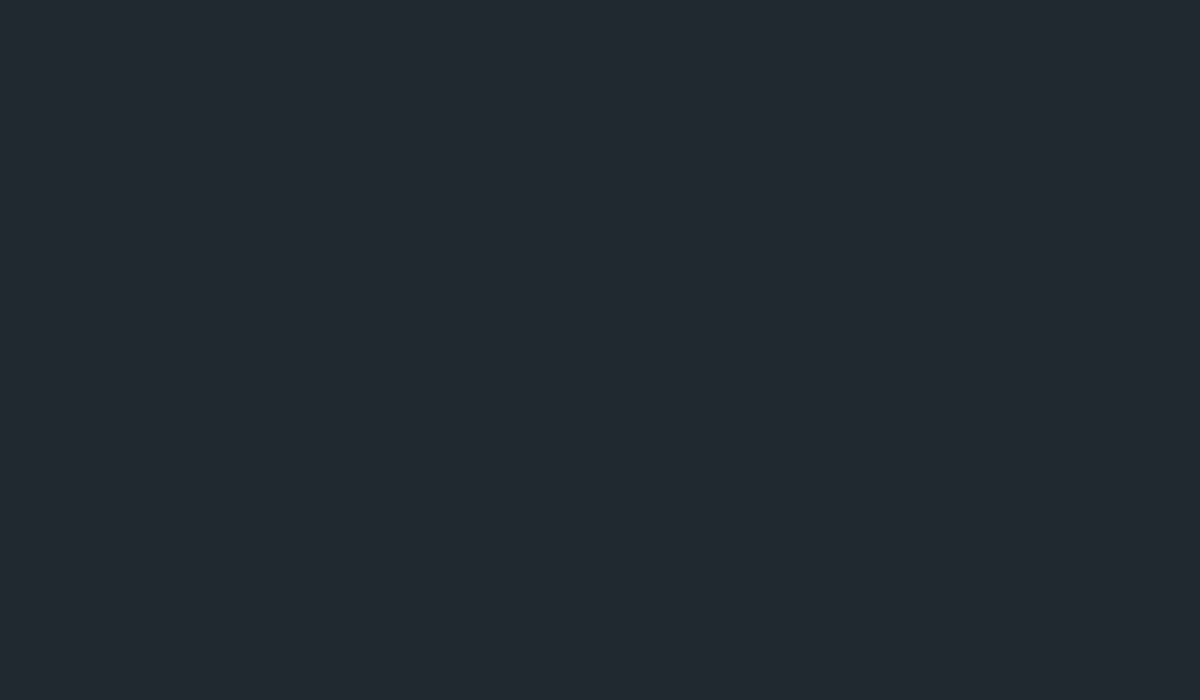
\includegraphics[width=0.92\textwidth]{poc-level-editor.png}
\caption[Level-scherm met editor en checklist]{Level-scherm met Monaco-editor, Python-referentie en checklist van doelen na validatie.}
\label{fig:poc-level-editor}
\end{figure}

\subsection{Voorbeeld: level~1 (divisions)}
De gebruiker moet onder meer de vier divisions en \texttt{STOP RUN.} bevatten.
Een minimaal geslaagd fragment ziet er conceptueel als volgt uit:

\begin{minted}[fontsize=\footnotesize,breaklines]{text}
       IDENTIFICATION DIVISION.
       PROGRAM-ID. HELLO.

       ENVIRONMENT DIVISION.

       DATA DIVISION.
       WORKING-STORAGE SECTION.

       PROCEDURE DIVISION.
           DISPLAY "OK".
           STOP RUN.
\end{minted}

\section{Gamificatie en motivatie}

\subsection{Punten en eerste-pogingbonus}
Een geslaagd level levert \textbf{100 basispunten} op.
Indien de \textbf{eerste} indiening voor dat level onmiddellijk slaagt---er was dus nog geen eerdere mislukte validatie binnen dezelfde poging-sessie---wordt een \textbf{bonus van 25 punten} toegekend.
De UI toont dit expliciet in de ondertitel van de viering (zie verder).
Herhaalt een gebruiker een reeds voltooid level, dan worden er geen extra punten meer bijgeschreven; de poging wordt wel gelogd in \texttt{level\_attempts}.

\subsection{Badges en mijlpalen}
Badge-metadata staat centraal in \texttt{badge\_definitions} (zie tabel~\ref{tab:schema-badge-definitions}); toekenningen gebeuren in \texttt{user\_badges}.
Naast de \textbf{zeven inhoudsbadges} (één per level-thema, gekoppeld aan \texttt{LEVEL\_TO\_BADGE} in de code) kent de PoC een reeks \textbf{combinatieregels} die bij een eerste succes op een level in één transactie worden geëvalueerd:
\begin{itemize}
    \item \textbf{Eerste poging-succes:} badges \texttt{perfect\_streak} (schone run) en \texttt{first\_try\_success}.
    \item \textbf{Voortgang:} badges wanneer minstens 1, 3 of alle 7 levels minstens één keer geslaagd zijn.
    \item \textbf{Punten:} mijlpalen op cumulatieve \texttt{total\_points} (onder meer 1000, 2500 en 5000).
    \item \textbf{Tempo:} ``speedrun''-badges als de tijd tussen \texttt{started\_at} en het succes onder een drempel ligt (30~s, 1~min, 5~min).
\end{itemize}
Op het dashboard en de badges-pagina tonen tooltips de tekst uit \texttt{how\_to\_earn}, zodat duidelijk is wat er nog te verdienen valt---dit ondersteunt \textit{development \& accomplishment} en ontdekkingsdrang binnen het Octalysis-kader.

\subsection{Viering na een voltooid level (\texttt{LevelCelebration})}
Bij de \textbf{eerste} succesvolle afronding van een level wordt een \texttt{celebrationTrigger} verhoogd; daardoor rendert de component \texttt{LevelCelebration} opnieuw en start de feedbacklus.

\paragraph{Confetti.}
De bibliotheek \textbf{canvas-confetti} vuurt \textbf{twee confetti-bursts} af met licht verschoven parameters (\texttt{particleCount}, \texttt{spread}, \texttt{origin.y}) en een korte pauze van ongeveer 280~ms ertussen.
Zo ontstaat een merkbare ``klap'' zonder de pagina lang te blokkeren; de confetti gebruikt een hoge \texttt{zIndex} zodat ze boven de rest van de UI verschijnen.

\paragraph{Ballonnen en tekst.}
Bovenop de confetti verschijnen \textbf{zeven abstracte ballonnen} (afgeronde kolommen met gradiëntkleuren uit een vast palet), elk met een licht \textbf{gestaggerde} start (\texttt{delayMs}) en willekeurig uiteenlopende horizontale positie afgeleid van de trigger.
Ze animeren met de CSS-keyframes \texttt{balloonPopUp}: kort inspringen van onder het scherm, uitzoemen naar volle grootte, daarna omhoog bewegen en uitfaden (ongeveer 900~ms per ballon).
De titel ``Level $n$ compleet!'' en de ondertitel met punten gebruiken de keyframe \texttt{confettiTextIn} (fade/slide-in over ongeveer 420~ms).

\paragraph{Duur en toegankelijkheid.}
De overlay bedekt het volledige scherm maar heeft \texttt{pointer-events: none}, zodat de gebruiker niet per ongeluk klikken blokkeert.
Na ongeveer \textbf{2400~ms} wordt de viering verborgen; de overlay blijft technisch aanwezig maar visueel weg.
Parallel verschijnt een \textbf{toast} ``Level voltooid'' met dezelfde punttekst als de ondertitel van de viering.

\begin{figure}[H]
\centering

\includegraphics[width=0.92\textwidth]{poc-celebration.png}
\caption[Visuele beloning na een level]{Na een geslaagd level: confetti (twee bursts), ballonnen-animatie en titel/ondertitel met behaalde punten.}
\label{fig:poc-celebration}
\end{figure}

\subsection{Overige micro-feedback}
\begin{itemize}
    \item \textbf{Pagina-ingang:} belangrijke schermen gebruiken een lichte \texttt{animate-fade-in} (CSS) zodat navigatie niet abrupt aanvoelt.
    \item \textbf{Mislukte submit:} checklist-items en optioneel een fout-detailpaneel geven structurele feedback zonder confetti.
    \item \textbf{Voltooid level:} onder de editor verschijnt een informatieve \texttt{Alert} dat het level af is maar dat oefenen met de code nog kan.
\end{itemize}

\begin{figure}[H]
\centering
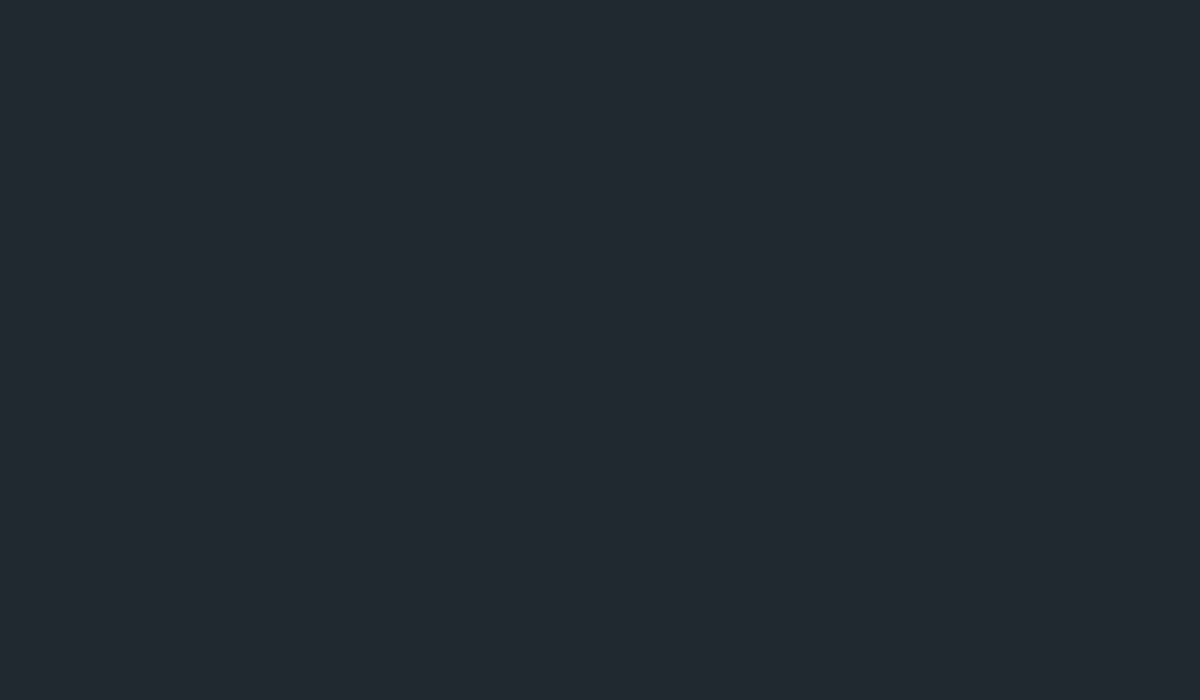
\includegraphics[width=0.92\textwidth]{poc-badges.png}
\caption[Badges-collectie]{Overzicht van beschikbare en behaalde badges met toelichting.}
\label{fig:poc-badges}
\end{figure}

\section{Leaderboard en vrienden}

\subsection{Rangschikking}
Het leaderboard rangschikt gebruikers op basis van onder meer totale punten en voltooide levels, met nadruk op de huidige gebruiker.
In ontwikkelmodus kunnen deterministische dummy-rijen worden toegevoegd om een lege ranking te vermijden; in productie worden uitsluitend echte profielen getoond.

\subsection{Realtime en sociale context}
Vriendenlijsten worden ververst bij login; waar relevant wordt real-time inschrijving op wijzigingen gebruikt zodat uitnodigingen en status sneller zichtbaar zijn.

\begin{figure}[H]
\centering
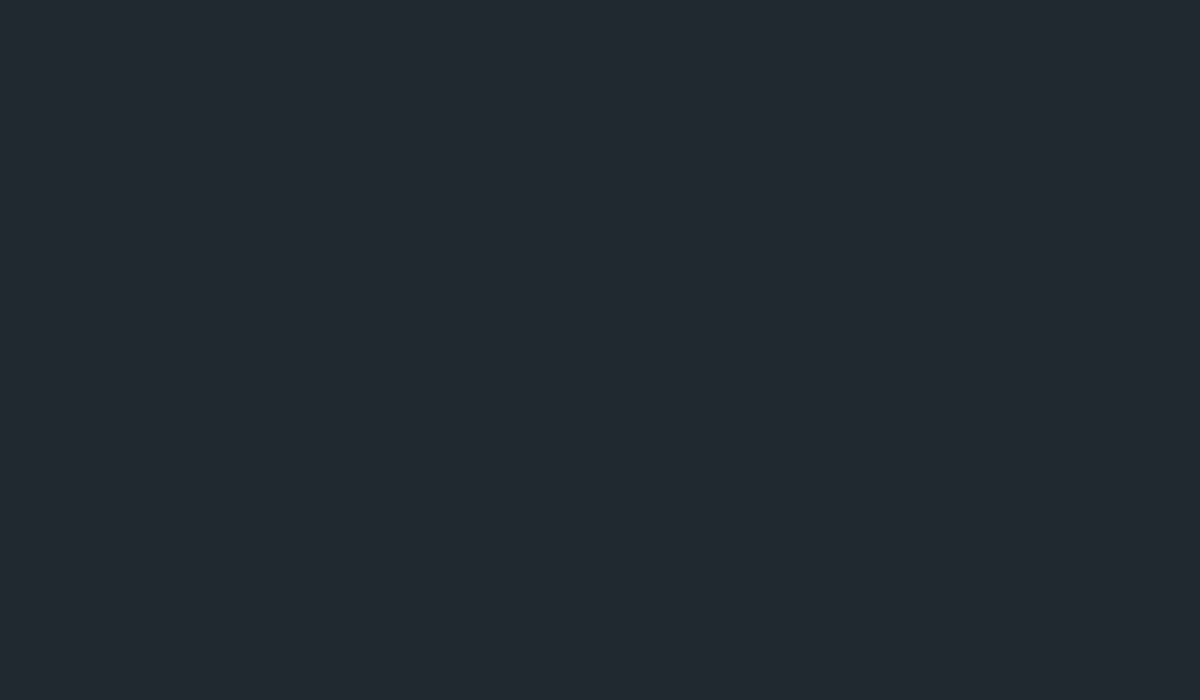
\includegraphics[width=0.92\textwidth]{poc-leaderboard.png}
\caption[Leaderboard]{Leaderboard met ranking, punten en voltooide levels.}
\label{fig:poc-leaderboard}
\end{figure}

\begin{figure}[H]
\centering

\includegraphics[width=0.92\textwidth]{poc-friends-profile.png}
\caption[Vrienden en profiel]{Vriendenfunctionaliteit en/of bezoek aan een vriendenprofiel.}
\label{fig:poc-friends-profile}
\end{figure}

\section{Gebruikersinterface: mainframe-esthetiek}

Visueel is gekozen voor een \textbf{donker thema}, monospace accenten en ``strip''-componenten die herinneren aan terminal- en mainframe-terminologie (\texttt{WORKING-STORAGE}, \texttt{ENVIRONMENT DIVISION}, enz.).
Dat draagt bij aan \textit{thema \& narratief} zonder een echte groene fosfor-CRT na te bootsen: leesbaarheid op moderne schermen blijft prioriteit (contrast, typografie, shadcn/ui-componenten).

\section{Samenvatting}

De PoC combineert een \textbf{gestructureerd leerpad} (zeven levels, sequentiële unlock), \textbf{Python-geankerde uitleg}, \textbf{directe checklist-feedback} op basis van heuristieken, en \textbf{gamificatie} (punten, mijlpaal- en speedrun-badges, confetti/ballon-viering, toasts, leaderboard, vrienden).
Technisch rust ze op React/TypeScript, Monaco, Supabase (zie het databasemodel in sectie~\ref{subsec:poc-db-schema}) en optionele Vercel-telemetrie.
De schermafdrukken in dit hoofdstuk illustreren de belangrijkste onderdelen van de PoC; vervang de bestanden in \texttt{graphics/} (repository-root) door scherpe exports van de uiteindelijke demo-omgeving vóór de finale indiening.

%%=============================================================================
%% Literatuurevaluatie van de PoC
%%=============================================================================

\chapter{\IfLanguageName{dutch}{Literatuurevaluatie van de Proof-of-Concept}{Literature-based evaluation of the Proof-of-Concept}}
\label{ch:evaluatie}

In dit hoofdstuk wordt de Proof-of-Concept uit hoofdstuk~\ref{ch:poc} geëvalueerd in twee delen.
Het eerste deel is een \emph{vergelijkende literatuurstudie} die in deze bachelorproef is uitgevoerd: elke ontwerpkeuze in \textit{Learn COBOL} wordt afgezet tegen empirische bevindingen over gamification, programmeeronderwijs en didactiek (secties~\ref{sec:evaluatie-methode}--\ref{sec:evaluatie-didactisch}).
Het tweede deel is een \emph{uitgewerkt onderzoeksdesign} voor een pilotstudie waarin de PoC empirisch wordt vergeleken met traditionele methoden zoals een papieren cursus met dezelfde leerthema's (sectie~\ref{sec:evaluatie-pilotstudie}).
Samen leveren beide delen een onderbouwd antwoord op de centrale onderzoeksvraag (sectie~\ref{sec:onderzoeksvraag}) en de deelvragen: de literatuurevaluatie op theoretische plausibiliteit, het pilotontwerp op hoe die plausibiliteit met deelnemers gemeten kan worden.

\section{Doel en aanpak van de evaluatie}
\label{sec:evaluatie-doel}

De evaluatie heeft drie concrete doelstellingen:
\begin{itemize}
    \item \textbf{Theoretische ondersteuning:} per gamification-element en per Octalysis Core Drive nagaan of de gemaakte ontwerpkeuze door de literatuur wordt ondersteund, gerelativeerd of tegengesproken.
    \item \textbf{Antwoord op de deelvragen, met name DV5:} inschatten in hoeverre \textit{Learn COBOL} plausibel effectiever is dan traditionele methoden zoals een papieren cursus, op basis van vergelijkbaar empirisch onderzoek.
    \item \textbf{Voorbereiding van empirische validatie:} een reproduceerbaar pilotontwerp vastleggen zodat de literatuurhypotheses later met deelnemers gemeten kunnen worden.
\end{itemize}

De koppeling met de deelvragen uit sectie~\ref{sec:onderzoeksvraag} is als volgt.
DV1, DV2, DV3 en DV4 worden inhoudelijk al beantwoord in respectievelijk hoofdstuk~\ref{ch:stand-van-zaken} en hoofdstuk~\ref{ch:poc}.
DV5 wordt in dit hoofdstuk beantwoord in twee stappen: eerst via de literatuurevaluatie (meta-analyse van \textcite{Zhan2022}, verschil tussen interactieve en statische leertools uit hoofdstuk~\ref{ch:stand-van-zaken}), daarna via het pilotontwerp dat beschrijft \emph{hoe} die vergelijking empirisch zou worden uitgevoerd.

\paragraph{Evaluatiestrategie: literatuurevaluatie en pilotontwerp}
\label{subsec:evaluatie-keuze}

De oorspronkelijke onderzoeksopzet voorzag een empirische vergelijking tussen de PoC en traditionele methoden zoals een papieren cursus: twee groepen deelnemers leren elk één dag COBOL, één groep via de PoC en één groep via een papieren cursus, en hun resultaten op dezelfde kennistest worden vergeleken.
Dat volledige onderzoek kon binnen het tijdsbestek van deze bachelorproef niet worden uitgevoerd.
Twee knelpunten bepaalden die keuze:

\begin{itemize}
    \item \textbf{Rekrutering en planning.} Voldoende deelnemers vinden die aan de inclusiecriteria voldoen vraagt veel screening. De doelgroep bestaat uit junior IT'ers met Python-ervaring én zonder enige COBOL-kennis. Voor een zinvolle spreiding wordt typisch \(N \geq 12\) als minimum gehanteerd.
    \item \textbf{Materiaal en uitvoering.} Een eerlijke vergelijking vereist een vooraf gevalideerde papieren cursus, screening, gestandaardiseerde instrumenten en voor elke deelnemer twee geplande sessies plus export van applicatielogs.
\end{itemize}

In plaats van een onderbouwde pilot met slechts twee of drie deelnemers uit te voeren, is gekozen voor een tweeledige aanpak.


Literatuurevaluatie (uitgevoerd): de ontwerpkeuzes van de PoC worden theoretisch \emph{gekalibreerd} tegen bestaande empirische literatuur.
Die stap levert geen causale claim over \textit{Learn COBOL} zelf, wel een conceptueel onderbouwde uitspraak: indien de PoC ingezet wordt zoals beschreven, is het op basis van vergelijkbaar onderzoek aannemelijk dat de gamification-elementen een positief effect hebben op motivatie en leerwinst.
Pilotontwerp: sectie~\ref{sec:evaluatie-pilotstudie} beschrijft een vergelijkend experiment in uitvoerbare vorm (doelgroep, steekproef, tijdslijn, meetinstrumenten en analyse), zodat een opvolger de empirische validatie kan overnemen zonder het onderzoeksplan opnieuw te moeten ontwerpen.

\section{Methode van de literatuurevaluatie}
\label{sec:evaluatie-methode}

De evaluatie volgt een eenvoudig drie-staps-protocol per ontwerpkeuze:

\begin{enumerate}
    \item Beschrijf de ontwerpkeuze in de PoC zoals geïmplementeerd (zie hoofdstuk~\ref{ch:poc}).
    \item Identificeer een empirische claim uit de literatuur die op die keuze van toepassing is.
    \item Beoordeel de uitlijning tussen de ontwerpkeuze en de claim: bevestigt de literatuur de keuze, zet ze die in perspectief, of waarschuwt ze ertegen?
\end{enumerate}

De voornaamste bronnen voor stap~2 zijn de meta-analyse van \textcite{Zhan2022} (over gamification in programmeeronderwijs), het werk van \textcite{KevinWerbach2020} (over de PBL-triade en haar valkuilen), het Octalysis-framework van \textcite{Chou2015}, het MDA-framework van \textcite{Hunicke2004}, het overzicht van \textcite{Cepeda2006} over het spacing effect en de marktanalyse van COBOL-leermiddelen uit hoofdstuk~\ref{ch:stand-van-zaken}.


\paragraph{Wat de literatuurevaluatie niet doet.}
Ze meet géén leeruitkomsten op deelnemers en levert dus géén testresultaten of andere directe metingen op gebruikers op.
De secties~\ref{sec:evaluatie-pbl}--\ref{sec:evaluatie-didactisch} geven per ontwerpkeuze een \emph{verwacht effect}, niet een gemeten effect op gebruikers van \textit{Learn COBOL}.

\section{Evaluatie van de PBL-elementen}
\label{sec:evaluatie-pbl}

Het protocol uit sectie~\ref{sec:evaluatie-methode} wordt hieronder toegepast op vier thema's: PBL, Octalysis, MDA en het didactische ontwerp.

De PoC implementeert de drie klassieke PBL-componenten: punten (met first-try bonus), badges (zeven inhoudsbadges, plus combinatiebadges rond clean run, mijlpalen en speedrun) en een leaderboard. 
\textcite{KevinWerbach2020} benadrukken dat PBL het \emph{startpunt} van gamification is, niet het eindpunt: enkel een dunne PBL-laag op een bestaand systeem leggen (de zogenaamde \textit{PBL-fallacy}) leidt zelden tot duurzame motivatie. 
De vraag is dus niet of PBL aanwezig is, maar of de drie elementen ingebed zijn in een breder ontwerp dat onderliggende motivatoren raakt.

\paragraph{Punten}
De PoC kent als beloning voor een geslaagd level 100 punten toe en geeft 25 bonuspunten wanneer de eerste indiening correct is. Deze keuze sluit aan bij wat \textcite{KevinWerbach2020} beschrijven als ``zinvolle'' puntenstructuren: punten zijn gekoppeld aan een concrete prestatie.
De first-try bonus maakt daarnaast gebruik van de Core Drive \textit{Loss \& Avoidance} \autocite{Chou2015}: door de bonus te missen verlies je een onmiddellijk zichtbaar voordeel, wat aanzet tot zorgvuldig lezen vóór indienen. 

\paragraph{Badges}
De PoC kent zeven inhoudsbadges (één per leerthema) plus combinatiebadges. 
Hiernaast is er een pagina waar gebruikers verdiende en nog te verdienen badges kunnen bekijken. Hier kunnen ze ook zien hoe ze de badge kunnen verdienen.
Dit komt overeen met de aanbevelingen van \textcite{KevinWerbach2020} dat badges twee functies moeten combineren: een erkenning- en een ontdekkingsfunctie.

\paragraph{Leaderboard}
Dit is het meest betwiste PBL-element. \textcite{KevinWerbach2020} waarschuwen expliciet dat leaderboards in zakelijke contexten kunnen demotiveren wanneer de afstand tot de top te groot is, en in extreme gevallen zelfs ongewenst gedrag kunnen uitlokken. 
De PoC mitigeert dit risico op twee manieren: het volledige leaderboard staat op een aparte route (\texttt{/leaderboard}), en het dashboard toont een ingekorte top-drie van vrienden in plaats van de globale top-N. 

\paragraph{Tussentijdse conclusie.}
De PBL-implementatie in \textit{Learn COBOL} vermijdt de PBL-fallacy door alle drie de elementen aan een bredere ontwerplaag te koppelen (zie sectie~\ref{sec:evaluatie-octalysis} en~\ref{sec:evaluatie-mda} hieronder).
De keuzes worden door de literatuur over PBL ondersteund.

\section{Evaluatie tegen het Octalysis-framework}
\label{sec:evaluatie-octalysis}

Het Octalysis-framework van \textcite{Chou2015} biedt acht \textit{Core Drives} (CD's) als checklist om te beoordelen of een gamified systeem gebalanceerd is.
Tabel~\ref{tab:eval-octalysis} koppelt elk Core Drive aan de concrete ontwerpkeuzes in de PoC.

\begin{table}[H]
\centering
\small
\begin{enumerate}[label=\textbf{CD\arabic*}, leftmargin=*, itemsep=0.55em, topsep=0.4em]
    \item \textit{Epic Meaning \& Calling}: mainframe-strips rond \texttt{WORKING-STORAGE} en \texttt{PROCEDURE DIVISION}; narratief dat COBOL kritieke infrastructuur draagt.
    \item \textit{Development \& Accomplishment}: levels, voortgangsbalk, checklist met vinkjes, punten, badges, viering bij succes, rang en tier op het profiel.
    \item \textit{Empowerment of Creativity \& Feedback}: vrije code-invoer met onmiddellijke validatie tegen leerdoelen.
    \item \textit{Ownership \& Possession}: profielpagina met avatar, cumulatieve punten en een badge-collectie gekoppeld aan het account.
    \item \textit{Social Influence \& Relatedness}: vriendenlijst, top-drie vrienden op het dashboard, volledig leaderboard op een aparte route, profielen van vrienden.
    \item \textit{Scarcity \& Impatience}: sequentiële ontgrendeling van levels, \textit{locked} badges blijven zichtbaar maar onbereikbaar.
    \item \textit{Unpredictability \& Curiosity}: optionele tips en documentatielinks per level; variatie in badge-eisen (speedrun, mijlpalen).
    \item \textit{Loss \& Avoidance}: bewust beperkt: geen ``levens'' of accountreset; enkel een first-try bonus die verloren kan gaan en lichte sociale vergelijking via het leaderboard.
\end{enumerate}
\caption{Mapping van Octalysis Core Drives op ontwerpkeuzes in \textit{Learn COBOL}}
\label{tab:eval-octalysis}
\end{table}

\paragraph{White hat / black hat balans.}
\textcite{Chou2015} adviseert een combinatie van \textit{White Hat} motivatoren (CD1, CD2, CD3: positief en versterkend) en \textit{Black Hat} motivatoren (CD6, CD7, CD8: gebaseerd op schaarste, nieuwsgierigheid en verliesangst). 
De PoC is duidelijk White-Hat-zwaar. Core Drives 1--3 (tabel~\ref{tab:eval-octalysis}) richten zich op voortgang, feedback en betekenis, terwijl CD6--CD8 bewust beperkt zijn ingezet. 

\paragraph{Verwachte effectgrootte.}
De meta-analyse van \textcite{Zhan2022} rapporteert voor gamification in programmeeronderwijs een gestandaardiseerd gemiddeld effect van ongeveer \(SMD = 0{,}77\) op studentmotivatie en \(\approx 0{,}75\) op academische prestaties, beide medium-tot-grote effecten. 
Aangezien de PoC alle door Zhan beschreven kerncomponenten (punten, badges, levels, directe feedback, sociale vergelijking) implementeert, is het aannemelijk dat een eventuele empirische test minstens binnen dezelfde grootteorde zou vallen. 
Deze voorspelling moet wel met voorbehoud gelezen worden: de meta-analyse aggregeert sterk uiteenlopende studies en contexten, en de overdraagbaarheid naar specifiek COBOL-onderwijs is niet getest.

\section{Evaluatie via het MDA-perspectief}
\label{sec:evaluatie-mda}

Het MDA-framework \autocite{Hunicke2004} dwingt om na te denken over hoe \textit{mechanics} (regels en code) zich vertalen in \textit{dynamics} (gedrag tijdens gebruik) en uiteindelijk in \textit{aesthetics} (de emotionele beleving).

\begin{itemize}
    \item \textbf{Mechanics:} validatiecode, puntberekening, sequentiële ontgrendeling.
    \item \textbf{Dynamics:} competitie om rang, het mikken op een first-try bonus, het vergelijken van eigen voortgang met die van vrienden, herhaalbaar oefenen van een level.
    \item \textbf{Aesthetics:} \textit{Challenge} (levels overwinnen) als dominante emotie, \textit{Fantasy} via het mainframe-thema en \textit{Narrative} via de strips.
\end{itemize}

De evaluatie levert hier vooral een kwalitatieve check op: zijn de mechanics ontworpen om de gewenste aesthetics te ondersteunen?
In de PoC zorgt de combinatie van checklist, voortgangsbalk en celebration-overlay ervoor dat \textit{Challenge} en de bijhorende beloning in dezelfde momenten gebeuren. 
Dit ontwerpprincipe, mechanics laten samenkomen naar één moment, is wat \textcite{Hunicke2004} ``the right kind of fun'' noemen.

\section{Evaluatie van het didactische ontwerp}
\label{sec:evaluatie-didactisch}

Naast de gamification-laag bevat de PoC een aantal expliciet didactische keuzes die los van Octalysis of MDA staan.

\paragraph{Heuristische validatie en checklistfeedback.}
De keuze om de PoC niet te koppelen aan een echte COBOL-compiler maar te valideren via regex-patronen op leerdoelen, levert twee voordelen op: feedback is direct (geen compilatietijd) en feedback is in dezelfde \emph{taal} geformuleerd als de opdracht (``alle vier divisions aanwezig'') in plaats van compilermeldingen die voor beginners cryptisch overkomen.
Onderzoek over interactieve programmeeromgevingen toont dat het type feedback minstens even belangrijk is als de aanwezigheid ervan: feedback die expliciet leerdoel-gericht is, wordt door beginners beter benut dan generieke foutmeldingen \autocite{Zhan2022}. 
De keerzijde is een verlies aan correctheidsgarantie: de PoC kan code goedkeuren die in een echte compiler zou falen.

\paragraph{Distributed practice en spacing effect.}
De levelstructuur met herhaalbare opdrachten, badge-eisen die meerdere bezoeken vereisen (bv.\ speedrun), en het feit dat een voltooid level later opnieuw kan worden geopend, ondersteunen distributed practice. 
\textcite{Cepeda2006} beschrijven in hun overzicht van het spacing effect dat leren over meerdere kortere sessies typisch betere lange-termijn retentie oplevert dan één blokje massaal oefenen. 
Een gamified leerpad met streaks, mijlpalen en herhaalbare levels is in dat opzicht een betere container voor verspreide oefening dan een statisch PDF-document, dat doorgaans één keer wordt doorlopen.

\section{Beperkingen van de literatuurevaluatie}
\label{sec:evaluatie-beperkingen}

De literatuur-gebaseerde resultaten in secties~\ref{sec:evaluatie-pbl}--\ref{sec:evaluatie-didactisch} hebben inherente beperkingen.
Die beperkingen zijn geen afwijzing van empirisch onderzoek, maar motiveren het pilotontwerp in sectie~\ref{sec:evaluatie-pilotstudie}.

\begin{itemize}
    \item \textbf{Geen empirische geldigheid voor de PoC zelf.} De resultaten ondersteunen de plausibiliteit van de ontwerpkeuzes, maar tonen niet aan dat \textit{Learn COBOL} in de praktijk een hogere leer-effectiviteit haalt dan een statisch alternatief.
    \item \textbf{Selectiebias in de literatuur.} De geraadpleegde meta-analyses focussen vooral op moderne talen (Python, Java, Scratch, \ldots). Of de gemeten effecten zich op dezelfde manier voordoen bij een verbose, decennia-oude taal als COBOL is niet onderzocht.
    \item \textbf{Confounding van interactiviteit en gamification.} De positieve effecten in \textcite{Zhan2022} ontstaan deels door interactiviteit op zich, niet enkel door gamification.
    \item \textbf{Heuristische validatie.} De PoC valideert COBOL-code via regex-patronen, niet via een echte compiler. False positives en false negatives zijn mogelijk.
\end{itemize}

\section{Ontwerp van een pilotstudie ter validatie van de PoC}%
\label{sec:evaluatie-pilotstudie}

De literatuurevaluatie levert plausibiliteit. Een empirische meting op echte deelnemers vereist het onderzoeksdesign dat hieronder wordt uitgewerkt.
Het plan sluit aan op de oorspronkelijke onderzoeksopzet (PoC versus papieren cursus, zelfde zeven leerthema's) en op de beperkingen uit sectie~\ref{sec:evaluatie-beperkingen}.

Onderstaand plan beschrijft een beknopte pilotstudie met een beperkte steekproef (\(N = 12\) tot \(20\)).
Het doel is na te gaan of de PoC tot betere leeruitkomsten leidt dan een klassieke aanpak na één leerdag.
De vergelijking gebeurt op één enkele kennistest die beide groepen maken na hun leerdag.

\subsection{Doelstellingen}

De pilot heeft één gericht doel: nagaan of de PoC tot betere leeruitkomsten leidt dan een klassieke aanpak na één leerdag.
Concreet wordt vergeleken hoe deelnemers die één dag met de PoC werken scoren op dezelfde kennistest als deelnemers die één dag met een papieren cursus werken, met dezelfde zeven leerthema's en volgorde als in hoofdstuk~\ref{ch:poc}.

\subsection{Doelgroep, inclusiecriteria en steekproef}

\textbf{Doelgroep:} junior developers of IT-studenten met een Python-basis en geen voorafgaande formele COBOL-opleiding.

\textbf{Inclusie:} zelfgerapporteerd voldoende Python om de parallelle voorbeelden te volgen, en bereidheid om één leerdag en aansluitend de kennistest af te leggen.

\textbf{Exclusie:} deelnemers aan een Mainframe-/COBOL-specialisatie, professionele COBOL-ervaring.

\textbf{Steekproefgrootte:} We streven naar \(N = 12\) tot \(20\) deelnemers in totaal, ongeveer 6 tot 10 per groep.

\subsection{Onderzoeksopzet}

Het ontwerp is tussen-proefpersoon. Dat wil zeggen dat elke deelnemer maar één van de twee leermethoden volgt, niet beide. Zo wordt vermeden dat de eerste methode de tweede meting beïnvloedt.

De deelnemers worden willekeurig verdeeld over twee groepen:
\begin{itemize}
    \item \textbf{Groep A (klassiek):} leert COBOL gedurende één dag met traditionele methoden zoals een papieren cursus die dezelfde zeven leerthema's behandelt als in hoofdstuk~\ref{ch:poc}.
    \item \textbf{Groep B (PoC):} leert COBOL gedurende één dag met \textit{Learn COBOL}, langs dezelfde zeven leerthema's in dezelfde volgorde.
\end{itemize}

Aan het eind van de leerdag maken beide groepen dezelfde kennistest over die zeven leerthema's. De primaire vergelijking is het gemiddelde testresultaat van groep A tegenover dat van groep B.

\subsection{Tijdslijn}

Figuur~\ref{fig:pilot-tijdlijn} geeft een relatieve tijdslijn van vijf opeenvolgende weken vanaf de start van de pilotvoorbereiding.

\begin{figure}[H]
\centering
\resizebox{\linewidth}{!}{%
\begin{tikzpicture}[
    font=\small,
    tick/.style={thick},
    lbl/.style={align=left, text width=3.15cm, inner sep=2pt}
]
    \coordinate (A) at (-0.15,0);
    \coordinate (END) at (14.25,0);
    \draw[tick,-{Latex[length=2.8mm]}] (A) -- (END);
    \foreach \x in {0, 4.05, 8.1, 11.6}
        \draw (\x,-0.17) -- (\x,0.17);
    \node[lbl, below=14pt] at (0,-0.17) {\textbf{Week~1}\\[3pt]
        Papieren cursus en kennistest afronden, informed consent opstellen, instrumenten testen buiten de steekproef.};
    \node[lbl, above=14pt] at (4.05,0.17) {\textbf{Week~2}\\[3pt]
        Screening van deelnemers en willekeurige toewijzing aan groep A of groep B.};
    \node[lbl, below=14pt] at (8.1,-0.17) {\textbf{Week 3--4}\\[3pt]
        Datacollectie: één leerdag per deelnemer in de toegewezen groep, gevolgd door de kennistest.};
    \node[lbl, above=14pt] at (11.6,0.17) {\textbf{Week~5}\\[3pt]
        Analyse, vergelijking van de testresultaten tussen beide groepen en pilotrapport.};
\end{tikzpicture}%
}%
\caption{Relatieve tijdslijn van de pilotfase}%
\label{fig:pilot-tijdlijn}
\end{figure}

\subsection{Meetinstrumenten}

\paragraph{Kennistest na de leerdag.}
Aan het eind van de leerdag legt elke deelnemer dezelfde kennistest af. Dat is een korte test met vragen over de zeven leerthema's uit tabel~\ref{tab:poc-levels}. Beide groepen krijgen exact dezelfde vragen, zodat de scores rechtstreeks vergelijkbaar zijn.

De primaire uitkomstmaat is het gemiddelde aantal correct beantwoorde vragen per groep. Het verschil tussen beide groepsgemiddelden geeft een indicatie van de leer-effectiviteit van de PoC ten opzichte van de klassieke papieren cursus.

%%=============================================================================
%% Conclusie
%%=============================================================================

\chapter{Conclusie}%
\label{ch:conclusie}

Deze bachelorproef onderzocht de centrale onderzoeksvraag uit sectie~\ref{sec:onderzoeksvraag}: \textit{``Hoe effectief is gamification bij het aanleren van COBOL aan junior developers die gewend zijn aan moderne talen zoals Python?''}
Om hierop een onderbouwd antwoord te formuleren, werd een literatuurstudie uitgevoerd (hoofdstuk~\ref{ch:stand-van-zaken}), een Proof-of-Concept ontwikkeld als interactieve webapplicatie (hoofdstuk~\ref{ch:poc}), en de PoC geëvalueerd in twee delen (hoofdstuk~\ref{ch:evaluatie}). Eerst via een uitgevoerde literatuurevaluatie. Daarna via een voorbereid maar niet uitgevoerd pilotontwerp voor een vergelijking met traditionele methoden zoals een papieren cursus.

\section{Antwoord op de onderzoeksvragen}

\begin{description}
    \item[DV1: uitdagingen in syntax en logica.] Inhoudelijk beantwoord in hoofdstuk~\ref{ch:stand-van-zaken} (sectie~\ref{sec:COBOL-versus-python}). Belangrijke verschilpunten voor een Python-georiënteerde junior zijn onder meer de \texttt{PIC}-clausule, de hiërarchische level-numbers, de scope-valstrik met de punt (\texttt{.}) en de verbose programmastructuur.

    \item[DV2: barrières bij het leren.] Beschreven in hoofdstuk~\ref{ch:stand-van-zaken}. Bovenop de syntactische verschillen geldt de \emph{didactische kloof}: het bestaande COBOL-leermateriaal is vooral statisch, terwijl de doelgroep gewend is aan interactieve sandboxes.

    \item[DV3: gamification-elementen.] De literatuur onderscheidt een bredere set gamification-\allowbreak elementen dan enkel de PBL-triade: prestatiebeloningen (punten, badges, mijlpalen), uitdagingselementen (levels en opdrachten), sociale elementen (leaderboards en vergelijking), narratieve/rol-\allowbreak elementen (thema, verhaal, avatars), en feedback- en progressie-\allowbreak elementen (onmiddellijke validatie, checklists, voortgangsbalken) \autocite{KevinWerbach2020, Chou2015}. Voor het leren van COBOL sluiten vooral drie categorie\"en het best aan: (1) uitdagingen met snelle feedback, (2) zichtbare prestatiebeloningen, en (3) herhaalbare oefening in een levelstructuur (distributed practice/spaced repetition). Die combinatie ondersteunt zowel \textit{Development \& Accomplishment} als \textit{Empowerment of Creativity \& Feedback} en past bij de specifieke leerdrempels van COBOL (strikte structuur, expliciete syntax en veel procedurele patronen), terwijl sociale competitie via leaderboards best beperkt en doordacht wordt ingezet omdat dit niet voor elke beginner motiverend werkt \autocite{Zhan2022, KevinWerbach2020, Cepeda2006}.

    \item[DV4: ontwerp van een gamified leeromgeving.] Concreet uitgewerkt in hoofdstuk~\ref{ch:poc}. De literatuurevaluatie in hoofdstuk~\ref{ch:evaluatie} linkt de belangrijkste ontwerpkeuzes aan onderzoek (punten en badges, leaderboard, Octalysis, MDA en didactische feedback). Daardoor is het ontwerp als geheel aannemelijk op basis van de geraadpleegde literatuur (secties~\ref{sec:evaluatie-pbl} tot~\ref{sec:evaluatie-didactisch}). De beperkingen daarvan staan expliciet in sectie~\ref{sec:evaluatie-beperkingen}.

    \item[DV5: leer-effectiviteit t.o.v.\ traditioneel.] Op basis van de literatuurevaluatie is het aannemelijk dat de gamification-elementen in \textit{Learn COBOL} een positief effect hebben op motivatie en leerwinst, in dezelfde grootteorde als de meta-analyse van \textcite{Zhan2022} rapporteert voor gamification in programmeeronderwijs (\(SMD \approx 0{,}77\) op motivatie, \(\approx 0{,}75\) op prestaties). Een rechtstreekse vergelijking met traditionele methoden zoals een papieren cursus is in deze bachelorproef niet getoetst; een definitief, kwantitatief antwoord op DV5 vraagt metingen met deelnemers. In sectie~\ref{sec:evaluatie-pilotstudie} staat daarvoor een pilotontwerp dat de leeruitkomsten van twee groepen vergelijkt, één die COBOL leert via de PoC en één die COBOL leert via een papieren cursus. Die pilot is in deze bachelorproef niet uitgevoerd.
\end{description}

\section{Bijdrage}

De toegevoegde waarde van dit onderzoek is viervoudig: een theoretisch kader dat gamification (PBL, MDA en Octalysis) koppelt aan mainframe-onderwijs; een functionele Proof-of-Concept op moderne webtechnologie (React, TypeScript, Supabase, Monaco) uitgewerkt in hoofdstuk~\ref{ch:poc}; een uitgevoerde literatuurevaluatie die per ontwerpkeuze onderbouwt waarom het ontwerp aannemelijk is; en een herbruikbaar pilotontwerp (sectie~\ref{sec:evaluatie-pilotstudie}) dat de stap naar empirische validatie concreet maakt.

\section{Aanbevelingen voor empirische opvolging}
\label{sec:conclusie-empirische-opvolging}

De voornaamste aanbeveling is de in hoofdstuk~\ref{ch:evaluatie} beschreven pilot daadwerkelijk uit te voeren. Dat is geen vervanging van de literatuurevaluatie, maar de volgende stap om de verwachtingen te toetsen met deelnemers en om voorzichtiger te kunnen spreken over oorzaak en overdraagbaarheid.
Het onderzoeksdesign staat al volledig uitgewerkt in sectie~\ref{sec:evaluatie-pilotstudie}: doelstellingen, doelgroep, een tussen-proefpersoon opzet met willekeurige toewijzing aan groep A (papieren cursus) of groep B (PoC), een tijdslijn van vijf weken, en een gedeelde kennistest aan het eind van de leerdag als hoofdmeting.
Wat in deze bachelorproef ontbreekt, is enkel de uitvoering met deelnemers.

%---------- Bijlagen -----------------------------------------------------------

\appendix

\chapter{Onderzoeksvoorstel}

Het onderwerp van deze bachelorproef is gebaseerd op een onderzoeksvoorstel dat vooraf werd beoordeeld door de promotor. Dat voorstel is opgenomen in deze bijlage.
Merk op dat de uitvoering op één belangrijk punt is geëvolueerd ten opzichte van het oorspronkelijke voorstel: de oorspronkelijk geplande gebruikersstudie met twee focusgroepen (referentie- en doelgroep) bleek binnen het tijdsbestek van de bachelorproef niet haalbaar (zie sectie~\ref{subsec:evaluatie-keuze}) en werd vervangen door een vergelijkende literatuurevaluatie waarin de ontwerpkeuzes van de PoC worden afgezet tegen bestaand empirisch onderzoek.

\input{../voorstel/voorstel-inhoud}

%%---------- Andere bijlagen --------------------------------------------------
%% Plan B3 (vergelijkende literatuurevaluatie) gebruikt geen aanvullende
%% studiematerialen. De skeleton-bestanden in bachproef/bijlagen/ (PDF-pack,
%% SUS-vragenlijst) staan op de plank voor wie later alsnog een empirische
%% opvolgstudie wil opzetten (zie sectie 'Aanbevelingen voor empirische
%% opvolging' in het Evaluatie-hoofdstuk).

%%---------- Backmatter, referentielijst ---------------------------------------

\backmatter{}

\setlength\bibitemsep{2pt} %% Add Some space between the bibliograpy entries
\printbibliography[heading=bibintoc]

\end{document}
